\documentclass[12pt]{pom_thesis}
\author{Alan Antonio Peral Ortiz}
\advisor{Shahriar Shahriari}
\title{The Parks Location Problem}
\usepackage{tikz}
\newcounter{mycount}
\newcounter{mycounter}

\tikzset{
	mygrid/.pic={
		  
\draw[step=1cm,color=gray] (-2,-2) grid (3,3);
    \node[fill=cyan] at (-1.5,2.5) {};
    \node[fill=cyan] at (0.5,2.5) {};
    \node[fill=cyan] at (-.5,.5) {};
    \node[fill=cyan] at (2.5,.5) {};
    \node[fill=cyan] at (-1.5,2.5) {};
    \node[fill=cyan] at (1.5,-.5) {};
    \node[fill=cyan] at (-1.5,-1.5) {};

\setcounter{mycount}{1}
\foreach \y in {+2.6,+1.6,.6,-.4,-1.4}
  \foreach \x in {-1.6,-0.6,.4,1.4,2.4}
    \node at (\x,\y)[anchor=north west] {\tiny\arabic{mycount}\addtocounter{mycount}{1}};


	},
	uncoloredgrid/.pic={
	\draw[step=1cm,color=gray] (-2,-2) grid (3,3);

\setcounter{mycounter}{1}
\foreach \y in {+2.6,+1.6,.6,-.4,-1.4}
  \foreach \x in {-1.6,-0.6,.4,1.4,2.4}
    \node at (\x,\y)[anchor=north west] {\tiny\arabic{mycounter}\addtocounter{mycounter}{1}};
	
	
	}
}



\begin{document}

\maketitle

\begin{abstract}In this paper we do a little bit.  We have yet to look at the real model. For now we have the toy example. Refer to chapter two.
\end{abstract}

\pagenumbering{roman}
\tableofcontents

\newpage
\pagenumbering{arabic}
% this is how you begin a chapter:
% the label is so that you can refer to it later
\begin{chapter}{Introduction}
\label{Intro}
\section{What is Operations Research?}

	We begin with a brief history of Operations Research (OR), which arose out of the conflict of World War II. There was a specific need to allocate scarce resources to military operations in an effective manner, and so the British and US militaries had scientists perform \textit{research on} (military) \textit{operations}. In essence, the goal was to make the war machine more efficient, and they succeeded. They developed effective ways to use the new radar technology, as well as came up with better ways to manage convoys and conduct antisubmarine operations [CITE INTRO TO OR BOOK]. 
	
	The success that OR saw in the war then encouraged interest in non-military applications of the field.
% more intro shit
	A cursory glance at a variety of introductory textbooks will reveal that there is a certain focus on private sector applications of the field [Should probably cite this claim]. These applications tend to be primarily concerned with profit maximization and other aspects of running a business. While these problems provide for some interesting mathematical formulations, the field's ability to 
	
	There is a subfield of the discipline called Community-Based Operations Research, which seeks to shift the focus of OR from profit maximization or cost-reduction to improving the quality of life within a community. One of the main advocates of the field and of this lens that focuses on people as opposed to money is Michael P. Johnson, who compiled a textbook containing a variety of case studies that can constitute ``Community-Based Operations Research." 
	
	One of these case studies presented is the problem of park location in Bogot\'{a}, Colombia.

In the introduction I will explain the history of operations research and how it tends to be most utilized in the private sector. I will detail the development of (and necessity for) community-based operations research, and then explain that I will be examining a particular case study: the problem of developing new public parks in Bogot\'a, Colombia. I will perhaps provide a literature review here, a roadmap of what I will cover in the rest of the thesis, and anything else that may fit and come to mind later.

\section{An Introduction to the Parks Location Problem}

	In rapidly developed urban areas and large cities, the presence of public parks, green spaces, and other recreational facilities has been associated with a marked improvement in quality of life, mental health, and general wellbeing [CITE SOURCE]. Knowing this, the city of Bogot\'{a} (Colombia), one of the largest cities in Latin America with a population of about eight million that is expected to reach ten million by 2025, has implemented a number of changes that include the recovery of public spaces and the improvement of public parks [CITE THE SOURCE]. 
	
	In 2006, the mayor and city council of Bogot\'{a} threw their support behind a sports and recreation master plan for the city. This plan indicated that by 2019 the city must reach a minimum level of $2.71$  $\textrm{m}^2$ of neighborhood park area per resident. It then became the \textit{Instituto Distrital de Recreaci\'{o}n y Deporte} (IDRD), or Recreation and Sports Institute of Bogot\'{a}'s job to implement the master plan. As such, the IDRD was faced with a monumental challenge: they had to execute the construction of numerous new parks and revitalize dilapidated public spaces in a manner that balanced the differing geographic, social, and economic needs of the city. 
	
	Because of the many needs they had to consider and due to the nature of the problem, this problem was then modeled in such a way that it became a multiobjective facility location problem, which we will examine in further detail at a later point. For now we begin to consider the model.
% you should close a chapter before beginning a new one!
\end{chapter}

\begin{chapter}{A Look at the Model}
\section{A Simplified Model}
\subsection{Setting up the Problem}

In this chapter I present a simplified version of the model. We will take a look at some simpler examples and gradually increase the complexity of our example until we arrive at the one presented in the paper. We begin with a $5\times5$ grid, which will represent our simplified fictional city. Each block represents a plot of land, which might either be empty or occupied. If it is occupied, this means that there are people living on the block. Otherwise, the lot is empty and it is a candidate parcel, to potentially be turned into a park. We number each block from one to $25$, and we have colored every candidate parcel cyan. We want to build one park, and so we can choose from amongst all they cyan parcels. This is shown in figure \ref{fig:grid1}. We note that every lot is the same size. We also define the service area of the candidate parcels to consist of all the populated blocks adjacent and diagonal to the candidate parcel. For example, candidate parcel one's service area will consist of the set $\{2,6,7\}$. In other words, if we built a park on candidate parcel one, then the visitors would be from \textbf{only} those three surrounding lots. The first question we are interested in asking then becomes: 
\begin{center}
\textbf{Which candidate parcel will maximize the geographical coverage, as measured by the service area of the parcel?}
\end{center}
\begin{figure}
 \caption{Our $5\times 5$ grid city}
 \centering
 \label{fig:grid1}
 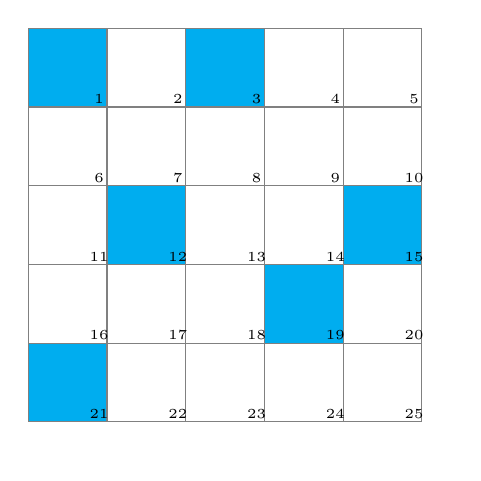
\begin{tikzpicture}[every node/.style={minimum size=1cm-\pgflinewidth}]
  \pic{mygrid};
\end{tikzpicture}
\end{figure}
In this example, it is possible to answer our question after merely observing the grid. Candidate parcel 12 would result in the highest number of lots served with 8. We now move on to defining a certain number of sets and variables so that we can present a mathematical formulation of the problem. \newline 
	
	We first let $\mathcal{J}$ be the set of all blocks that would benefit from the construction of a new park. Looking back to figure \ref{fig:grid1}, we see that $\mathcal{J} = \{ 2,4,6,7, \dots, 22, 23, 24, 25\}$. The candidate parcels have not been included in this set, and in this case we note that lot five is not included in $\mathcal{J}$ either because it is outside the service area of every candidate parcel. We also then define the set $\mathcal{I}$ to be the set of candidate parcels. In our case, $\mathcal{I} = \{ 1,3,12,15,19,21\}$. We finally define the set $\mathcal{W}_j$ for $j in \mathcal{J}$, which consists of all the candidate parcels that service block $j$. In our example, $\mathcal{W}_7 = \{1,3,12\}$. \newline
	
	We now define $z_j$ as a binary decision variable, taking on the value 1 if block $j \in \mathcal{J}$ is covered by at least one park, and 0 otherwise. So if we decided to build a park on candidate parcel 21, then $z_{16} = z_{17} = z_{22} = 1$, and for every other possible value of $j$ we would have $z_j = 0$. We also define the binary decision variable $y_i$, which will take on value 1 if candidate parcel $i$ is selected to become a park, and 0 otherwise. If we turned candidate parcel 21 into a park, then $y_{21} = 1$. We can now formulate our initial model:
\begin{align*}
\textrm{max } f_1 &= \sum_{j \in \mathcal{J}} z_j \\
\textrm{subject to } z_j &\leq \sum_{i \in \mathcal{W}_j} y_i, j \in \mathcal{J}\\
\left|\mathcal{W}_j\right|z_j &\geq \sum_{i \in \mathcal{W}_j} y_i, j \in \mathcal{J} \\
z_j &\in \{0,1\}, j \in \mathcal{J} \\
y_i &\in \{0,1\}, i \in \mathcal{I}
\end{align*}

	Our objective function seeks to maximize the geographical coverage of the potential parks to be built. The first constraint guarantees that if block $j$ is covered, then at least one parcel servicing it has been selected as a park. Conversely, the second constraint guarantees that if block $j$ is not covered, then none of the candidate parcels servicing it should be selected as parks. While I have referred to these first two constraints as being one constraint, the observation can be made that they must be satisfied for all values of $j \in \mathcal{J}$. An expansion of the model above to include all true constraints would like like so:
	\newline\newline
 \textbf{Here I was thinking of maybe typing out ALL of the model with all 40 constraints or so}
	\newline\newline
	  The last two constraints define our $z_j$ and $y_i$ as binary decision variables.

	As was mentioned earlier, wanting to select only one candidate parcel will result in the selection of candidate parcel 12. What if we wanted to build two parks? Looking at figure \ref{fig:grid2} we see that picking the two green parcels would result in a total coverage area of 13 blocks, which is the maximum in this case with two candidate parcels. 
	\begin{figure}
	\centering
	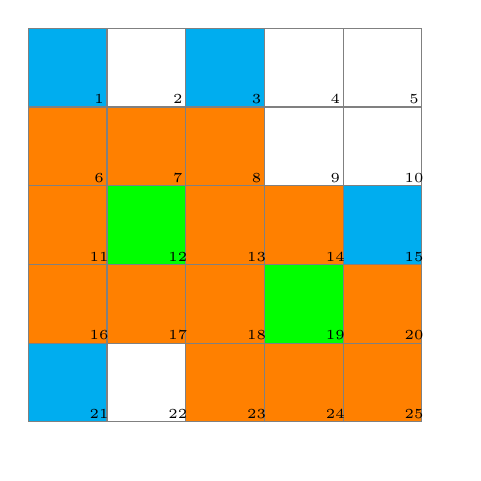
\begin{tikzpicture}[every node/.style={minimum size=1cm-\pgflinewidth}]
	\label{fig:grid2}
	\draw[step=1cm,color=gray] (-2,-2) grid (3,3);
   \node[fill=cyan] at (-1.5,2.5) {};
    \node[fill=green] at (-.5,.5) {};
     \node[fill=cyan] at (0.5,2.5) {};
    \node[fill=cyan] at (-1.5,2.5) {};
    \node[fill=cyan] at (2.5,.5) {};
    \node[fill=green] at (1.5,-.5) {};
    \node[fill=cyan] at (-1.5,-1.5) {};
    \node[fill=orange] at (-1.5,1.5){};
     \node[fill=orange] at (-1.5,.5){};
     \node[fill=orange] at (-1.5,-.5){};
     \node[fill=orange] at (-.5,1.5){};
     \node[fill=orange] at (-.5,-.5){};
     \node[fill=orange] at (0.5,-.5){};
      \node[fill=orange] at (.5,.5){};
       \node[fill=orange] at (.5,1.5){};
       \node[fill=orange] at (1.5,.5){};
       \node[fill=orange] at (.5,-1.5){};
        \node[fill=orange] at (1.5,-1.5){};
         \node[fill=orange] at (2.5,-1.5){};
         \node[fill=orange] at (2.5,-.5){};
   
\setcounter{mycount}{1}
\foreach \y in {+2.6,+1.6,.6,-.4,-1.4}
  \foreach \x in {-1.6,-0.6,.4,1.4,2.4}
    \node at (\x,\y)[anchor=north west] {\tiny\arabic{mycount}\addtocounter{mycount}{1}};
	\end{tikzpicture}
	\caption{Picking two candidate parcels to maximize geographical coverage.}
	\end{figure}
	
	
	We were able to see this result without having to do any calculations because of the simplicity of our model. But this is not always so apparent. We now begin to add layers of complexity to our model.
	
\subsection{Complicating the model}

We were previously only concerned with maximizing the geographical coverage of our model. In real life, prioritizing the geographical coverage of the potential parks serves to spread out the location of the parks and avoids building excessive parks in densely populated areas. It also proactively places in parks that may have yet to be developed or may be susceptible to rapid population growth in the future. However, we do not want to fully neglect the population density of the various city blocks. How does our model change when we add the number of inhabitants in each block? The question we are interested now becomes:
\begin{center}
\textbf{How do we maximize the geographical coverage of the parks as well as the number of beneficiaries that would result from the construction of the parks?}
\end{center}

We define the number of beneficiaries from a park construction as the sum of the population of all the blocks in the new park's service area. 

\begin{figure}
	\centering
	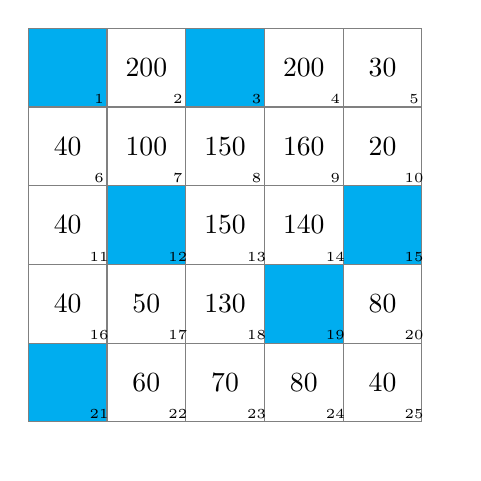
\begin{tikzpicture}[every node/.style={minimum size=1cm-\pgflinewidth}]
	\draw[step=1cm,color=gray] (-2,-2) grid (3,3);
   \node[fill=cyan] at (-1.5,2.5) {};
    \node[fill=cyan] at (-.5,.5) {};
     \node[fill=cyan] at (0.5,2.5) {};
    \node[fill=cyan] at (-1.5,2.5) {};
    \node[fill=cyan] at (2.5,.5) {};
    \node[fill=cyan] at (1.5,-.5) {};
    \node[fill=cyan] at (-1.5,-1.5) {};
    \node at (-1.5,1.5){40};
     \node at (-1.5,.5){40};
     \node at (-1.5,-.5){40};
     \node at (-.5,2.5){200};
     \node at (-.5,1.5){100};
     \node at (-.5,-.5){50};
     \node at (0.5,-.5){130};
      \node at (.5,.5){150};
       \node at (.5,1.5){150};
       \node at (1.5, 1.5){160};
       \node at (2.5, 1.5){20};
       \node at (2.5,2.5){30};
       \node at (1.5,2.5){200};
       \node at (1.5,.5){140};
       \node at (-.5,-1.5){60};
       \node at (.5,-1.5){70};
        \node at (1.5,-1.5){80};
         \node at (2.5,-1.5){40};
         \node at (2.5,-.5){80};
   
\setcounter{mycount}{1}
\foreach \y in {+2.6,+1.6,.6,-.4,-1.4}
  \foreach \x in {-1.6,-0.6,.4,1.4,2.4}
    \node at (\x,\y)[anchor=north west] {\tiny\arabic{mycount}\addtocounter{mycount}{1}};
	\end{tikzpicture}
	\caption{City blocks with population numbers.}
	\label{fig:gridpop}
	\end{figure}
	
	We now turn to figure \ref{fig:gridpop} to see an updated version of our model city. The residential blocks have been updated with a number that indicates the number of people living in that city block. This allows us to calculate the number of beneficiaries that would result from the construction of a park on any candidate parcel. Building a park on candidate parcel 21, for example, would result in 150 beneficiaries. We define one additional variable.
	
	Let $p_i$ to be the number of beneficiaries from candidate parcel $i$. In the example of parcel 21, we would have $p_{21} = 150$. We can now update our model:

\begin{align*}
\textrm{max } f_1 &= \sum_{j \in \mathcal{J}} z_j \\
\textrm{max } f_3 &= \sum_{i \in \mathcal{I}} p_iy_i \\
\textrm{subject to } z_j &\leq \sum_{i \in \mathcal{W}_j} y_i, j \in \mathcal{J}\\
\left|\mathcal{W}_j\right|z_j &\geq \sum_{i \in \mathcal{W}_j} y_i, j \in \mathcal{J} \\
z_j &\in \{0,1\}, j \in \mathcal{J} \\
y_i &\in \{0,1\}, i \in \mathcal{I}
\end{align*}

	Our model now has two objective functions. The first still seeks to maximize the geographical coverage of the parks. The second seeks to maximize the number of beneficiaries. But how do we maximize two things at the same time? We cannot guarantee that there will be a solution that maximizes the number of beneficiaries and the geographical coverage simultaneously. If we consider individual parcels, we notice that candidate parcel 3 serves the most amount of people, with $f_3 = 710$. However, candidate parcel 12 still has the most expansive geographical coverage, with $f_1 = 8$. How do we reconcile these two solutions?

\subsection{A Solution Strategy}

	We implement a lexicographic ordering of the objectives. In the real model, city planners from Bogot\'{a} ranked their priorities when it came to park placement. These priorities are reflected by the subscripts of the objective functions. Geographical coverage was deemed the most important criterion, so it is labeled $f_1$. Maximizing the number of beneficiaries was likewise deemed the third-most important criterion, so it is accordingly labeled $f_3$. There are two stages to solving this model, as developed by the mathematicians working on this project. The first stage involves solving for each objective function independently, with the given constraints.
	
	We will discuss the second stage at a later date.
\end{chapter}

\begin{chapter}{Multiobjective Facility Location Problems}
\section{What?}
Here we will look at the general class of Multiobjective facility location problems, which is the class of problems that contains the main model/problem I will be looking at for my thesis. 
\end{chapter}

\begin{chapter}{Discrete Facility Location Problems}
\section{What? pt. II}
The problem I will be examining also falls under this category. I am not sure how much this would vary from the previous chapter. But if it turns out there is a significant difference between both types of problems, it might be helpful to provide a dedicated chapter for both. Maybe the only difference is that the other class of problems has many objective functions.
\end{chapter}

\begin{chapter}{Applications}
If I have time to apply what I have learned to another problem, maybe this will go here. But this may be a bit ambitious. Stay tuned.
\end{chapter}

\end{document}

 